\begin{center}
\bd {\large {Триганометрическая запись комплексного числа}} \\
\end{center}

Декартова или прямоугольная система координат удобна для графических изображений
двумерных векторов. \\
\kv {Горизонтальная ось - действительная} \\
\kv {Вертикальная ось - мнимая (пишут значение i)} \\

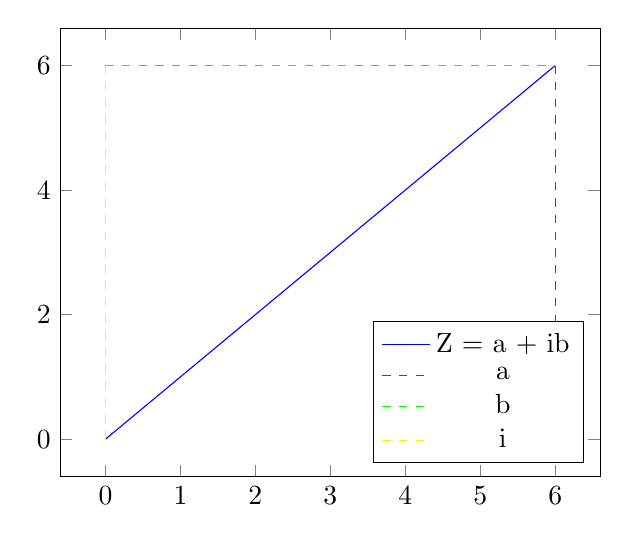
\begin{tikzpicture}
\begin{axis}[legend pos = south east]
\legend{Z = a + ib, a, b, i}
\addplot [solid, draw = blue] coordinates {
	(0,0) (6,6)
};

\addplot [dashed, draw = red] coordinates {
(6,0) (6,6)
};

\addplot [dashed, draw = green] coordinates {
(0,6) (6,6)
};

\addplot [dashed, draw = yellow] coordinates {
(0,0) (0,6)
};

\end{axis}
\end{tikzpicture}

$Z = a + ib \\
Z = (a; b)$ - векторное представление \\
В декартовой системе координат хорошо моделировать сложение комплексных чисел 
(сложение векторов) \\

\bd {Определение} \\
Полярная система координат называется направленный луч, с началом в точке \kv 
{О}, которое называется началом координат. \\
Если \kv {Z} - точка, то она определяется углом $\varphi$, который 
отсчитывается от оси против часовой стрелки $\varphi \in [0; 2 \Pi]$ и длиной 
радиуса вектора $\rho$. \\
В итоге точка координат определяется $(\varphi, \rho)$ \\

Чтобы установить связь между полярной и декартовой системой координам, 
совместим на рисунке обе системы координат \\

Пусть даны полярные координаты. Выразим через низ декартовые координаты. \\
$a = \rho \cdot cos\varphi$ \\
$b = \rho \cdot sin\varphi$ \\
Триганометрическая запись комплексного числа $Z = \rho (cos\varphi + i \cdot sin
\varphi)$ \\
Пусть даны декартовые координаты, выразим полярные. \\
$Z = a + ib \\
\rho = \sqrt{a^2 + b^2} \\
sin \varphi = \frac {b}{\sqrt{a^2 + b^2}} \\
\varphi = arcsin \frac {b}{\sqrt{a^2 + b^2}}$ \\

\bk {Также необходимо знать, чему равен косинус, чтобы определить в какой 
четверти лежит угол} \\

\bd {\large {Применение геометрической записи}} \\
\[Z_{1} = \rho_{1} (cos\varphi_{1} + isin\varphi_{1})\] \\
\[Z_{2} = \rho_{2} (cos\varphi_{2} + isin\varphi_{2}\] \\
\[Z_{1} \cdot Z_{2} = \rho_{1} \cdot \rho_{2} (cos\varphi_{1} \cdot cos\varphi_
{2} - sin\varphi_{1} \cdot sin\varphi_{2} + i(cos\varphi_{1} \cdot sin\varphi{2}
+ cos\varphi_{2} \cdot sin\varphi_{1})) = \] \\
\[ = \rho_{1} \cdot \rho_{2} (cos(\varphi_{1} + \varphi_{2}) + i \cdot sin
(\varphi_{1} + \varphi_{2})\] \\

\bd {\large {Геометрический смысл умножения}} \\
\bk{При умножении комплексных числе - их модули перемножаются, а углы складываются.} \\
Допустим мы хотим найти степени комплексного числа
